% !TeX spellcheck = en_GB 

\documentclass[a4paper, 10pt]{article}

\usepackage[english]{babel}
\usepackage[utf8]{inputenc}
\usepackage[pagestyles]{titlesec}
\usepackage{titletoc}
\usepackage{enumitem}
\usepackage{fancyhdr}
\usepackage[a4paper, margin = 2.5cm, headheight=14pt]{geometry}
\usepackage[hidelinks, colorlinks = false]{hyperref}
\usepackage[bottom]{footmisc}
\usepackage{bookmark}
\usepackage{fontspec}
\usepackage{graphicx}
\usepackage[labelfont = bf]{caption}
\usepackage{etoolbox}
\usepackage{tabularx}
\usepackage{colortbl}
\usepackage{float}

\usepackage[table]{xcolor}

\date{}

\title{
	
\includegraphics[width=0.75\textwidth]{assets/logo.png}
	\\
	{\huge Hubbl, a gym bookings manager}
}
\author{Miquel de Domingo i Giralt}

\setmainfont{Inter}[BoldFont = Inter Bold]
\setmonofont[Scale=0.9]{JetBrains Mono}

\newfontfamily\semibf{Inter Semi Bold}

% Variable with the page that keeps the footer style
\def\footerstyle{- \fontsize{10pt}{10pt}\selectfont\thepage\ -}
\pagestyle{fancy}
% Remove the horizontal bar from the header
\renewcommand{\headrulewidth}{0pt}
% Clear everythihg
\fancyhf{}
% Set header style
\rhead{\small\textit{\nouppercase{\rightmark}}}
% Set the footer page number
\fancyfoot[C]{\footerstyle}
% Update the footer in chapter and other plain views
\fancypagestyle{plain}{%
    \renewcommand{\headrulewidth}{0pt}%
    \fancyhf{}%
    \fancyfoot[C]{\footerstyle}%
}

\setlength\parindent{0pt}
\setcounter{secnumdepth}{5}
\setcounter{tocdepth}{5}

% Tables format
\definecolor{rowColor}{RGB}{242, 242, 242}	
\renewcommand{\arraystretch}{1.5}

\titleformat{\chapter}[hang]{\normalfont\huge\bfseries}{\thechapter. }{4pt}{\Huge}
\titlespacing{\chapter}{0pt}{-32pt}{12pt}

\begin{document}
\maketitle
\newpage
\section{Introduction}
On November 2019 the first cases of a new virus were coming into light. With similar symptomps as a regular flu, nobody would have imagined that the humanity would be at the edge of collapsing. The weeks went by and within few months, most countries of the world were completely shut down. It was not until the summer that people was able to go outside, again. Restaurants, hotels and any business that relied on the clients for their survival, had to face many restrictions imposed by the governors. One of such business where the gyms. The owners had to limit the total capacity of their installations and classes. Most companies had to find a new system which helped them handle appointents, since nearly any of them had an appointment system integrated in their respective applications.
\section{Project goals}
The goal of this final degree project is to develop a full stack application, which includes:
\begin{enumerate}[label = -]
	\item Designing the database.
	\item Implementing an API in order to interact with the database.
	\item Briefly designing the user interface.
	\item Implement the required front end applications, web based, in order to access the system.
\end{enumerate}
Fundamentally, the hubbl application will allow the creation of gym zones, which are explained in the next sections, which will allow the clients to create the needed appointments.
\\
As a future implementation yet not being a priority, the system will also have:
\begin{enumerate}[label = -]
	\item An analytics page which would provide information about the statistics of the gym.
	\item A subscription system for the clients.
\end{enumerate}
\section{Functionalities}
\subsection{Product description}
The product will provide a rich interface for the gym owners and their coworkers in order to manage their gym. Managers will create virtual gyms, each of one with different constrains, which will be forwarded to their gym zones. Each gym zone will be of a certain type, for example, a cardio zone, a free-weight zone or even a powerlifting zone. Such and more characteristics will be determined by the workers or who is responsible for the creation of the zones. Once determined the capabilities of each zone, the clients will have the possibility to make their reservations.
\\
This software is going to be interesting since it is mainly focused on the managing of appointments. There exist multiple manager systems, some are gym-focused yet there are few that provide an exclusive focus to managing the appointments. It is interesting to have an application that is that specific because most of the companies already have their client management system and other tools. The COVID has changed many things extremely fast and some gymnasiums have not been able to adapt fast enough. That is because using other management tools would mean to change the entire managing software of the company, in order words, starting from zero again. In the future, however, it would be nice to provide a client management system aswell, including subscriptions and so on.
\subsection{User needs: Owner or worker}
Such persona needs entire access to the management system, and it is the main user of it. For this persona, the following needs can be defined:
\begin{enumerate}[label = -]
	\item \emph{Ability to create virtual gyms and gym zones}. It is the main purpose of the application. It has to provide all the tools that are required to have an above average managing system.
	\item \emph{Modify virtual gyms and gym zones}. Constraints may change during time. Overall capacity may increase, more cardio machines may be added, and, with these changes, the gym zones will have to adapt to such real life modifications. There has to exist an interface that provides an easy and simple tool to control it.
	\item \emph{Ability to manage clients}. The income of the gym is based on the amount of clients they have, and such clients have to be subscribed into the system. However, the application is not a client management system. It purely focuses on the fact of appointments, yet the client still has to be registered in the application.
	\item \emph{Ability to manage appointments}. The workers have to be able to create, modify or delete the appointments at any time. This process has to be fast and simple, since it is more than usual to have cancellations, clients without reservation, and many more.
	\item \emph{Ability to manage guided events}. Some gym zones will be marked as a guided class zone. Therefore, a schedule will have to be set up for such zone in order to let the user know that.
\end{enumerate}
Furthermore, two user profiles have to be differentiated: the \emph{owner} and the \emph{worker}. The owner needs more control than the worker and some additional needs are\footnote{Some workers may also have access to such capabilities, depending on the permission they have recieved by the owner.}:
\begin{enumerate}[label = -]
	\item \emph{Ability to manage workers}. The owner has to be able to add, remove or update their workers. There must exist an interface that allows such control.
	\item \emph{Ability to manage the privileges of the workers}. In large gymnasium franchises, there may exist different types of workers, each with different tasks. For instance, some may only be able to manage guided sessions, others will manage the client subscriptions and so on. Therefore, a privilege system is required to define a hierarchy in the company.
	\item \emph{Ability to manage gym trainers}. It is important to know what trainers will be responsible for each guided class. For instance, some clients may prefer some trainers than others, when choosing a guided class.
\end{enumerate}
\subsection{User needs: Client}
The client has little interaction with the system. However, a management application for clients would be pointless if clients could not book their sessions. That is why it will exist another platform to provide access to the client. Such client, will have the following needs:
\begin{enumerate}[label = -]
	\item \emph{Ability to create, modify and delete appointments}. The clients will make the most use of the reservation system. There has to exist a simple and intuitive interface that allows the clients to interact with the system.
	\item \emph{Ability to visualise guided events}. In case the client prefers booking a place for a guided class, it should be able to visualise all the possible events for a day or week, for a zone.
\end{enumerate}
% IF MORE INFORMATION IS REQUIRED, ADD THE PRODUCT FUNCTIONALITIES SECTION
\section{Development methodology}
To structure and organise the project, working packages have been used in order to ensure a temporised and structured development. Following such structure has been extremely useful to simplify how are tasks managed and temporised. In order to organise the tasks, an \emph{AGILE} approach has been used, even though the project has been done all by myself. Each subgroup of the \emph{development} branch has been considered as an \emph{epic} and each working package as a \emph{story}, which has as many tasks as required. This approach has been used for each project and has made the development of the project easier to manage.
\\
In order to simplify the process of \emph{epic}, \emph{story} and \emph{task} creation, the Jira software from Atlassian has been used. It has been extremely useful as it can be integrated with many tools, one being GitHub, where the code is hosted. Using these elements, I have been able to automate the process of starting and completing tasks, alongside of the Jira automation. The following diagram, describes the workflow of the tasks inside Jira:
\begin{figure}[H]
	\centering
	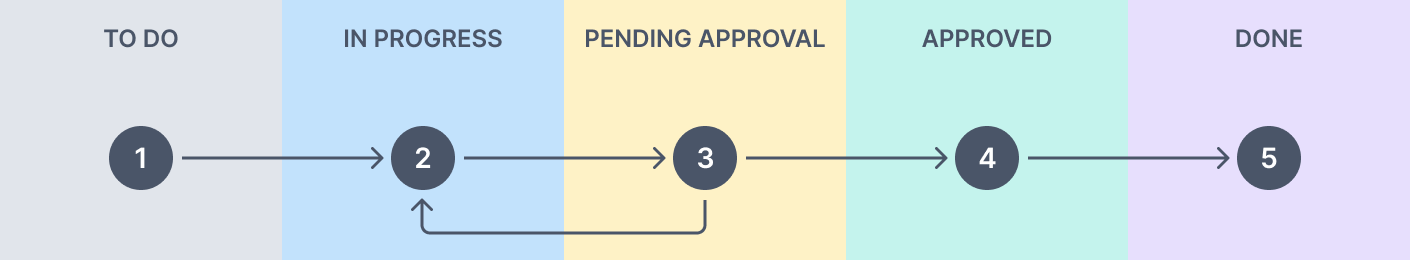
\includegraphics[width=\textwidth]{assets/working-packages/JiraWorkflow.png}
	\caption{5 steps of the Jira workflow}
\end{figure}
All the tasks would have to go from step 1 to step 5 in order to be considered as finished. Each step and the automation is as follows:
\begin{enumerate}
	\item All the tasks that have been selected for the sprint start at the first step, at the \emph{to-do} column.
	\item For each task, a new git branch has to be created with the name of the Jira task tag, for instance \texttt{HBL-185}\footnote{The \texttt{HBL} prefix is assigned when a new Jira project is created.}. When the branch is created and pushed to GitHub, Jira will move the task automatically to the \emph{in progress} column.
	\item While in progress, each commit made is tracked in Jira. Additionally, Jira also supports \emph{smart commits} which are words prefixed with a hash (\#). With the smart commits, task properties can be changed. In this case, only the \texttt{\#time} has been used which increments the amount of time spent in each task. Tracking time has been useful to know more precisely how much time has been spent overall.
	\item Once the task is finished, a new pull request is made which triggers the continuous integration workflows set up at the GitHub repository. These workflows can also be watched by Jira and automate operations in function of the workflow result. If the task does not pass one of the workflows, the task is moved back to the \emph{in progress} tab. Alternatively, if the checks pass, it is moved to the \emph{approved} column.
	\item Finally, in order to be considered \emph{done}, the pull request of the task in question has to be merged. The merge will trigger another automated process which moves the task from \emph{approved} to \emph{done}.
\end{enumerate}
In order to stick to the process as much as possible, tasks moved to \emph{done}, should not be moved back. Instead, a new \emph{bug} type task was created which would start the process again.
\\
In relation to the environment process, the project has been built using TypeScript, from the server to the different UI applications. The environment has been created using a monorepo build tool called Nx, which simplifies the monorepo management for JavaScript projects.
\subsection{Final product}
Here are some images of the core application:
\begin{figure}[H]
	\centering
	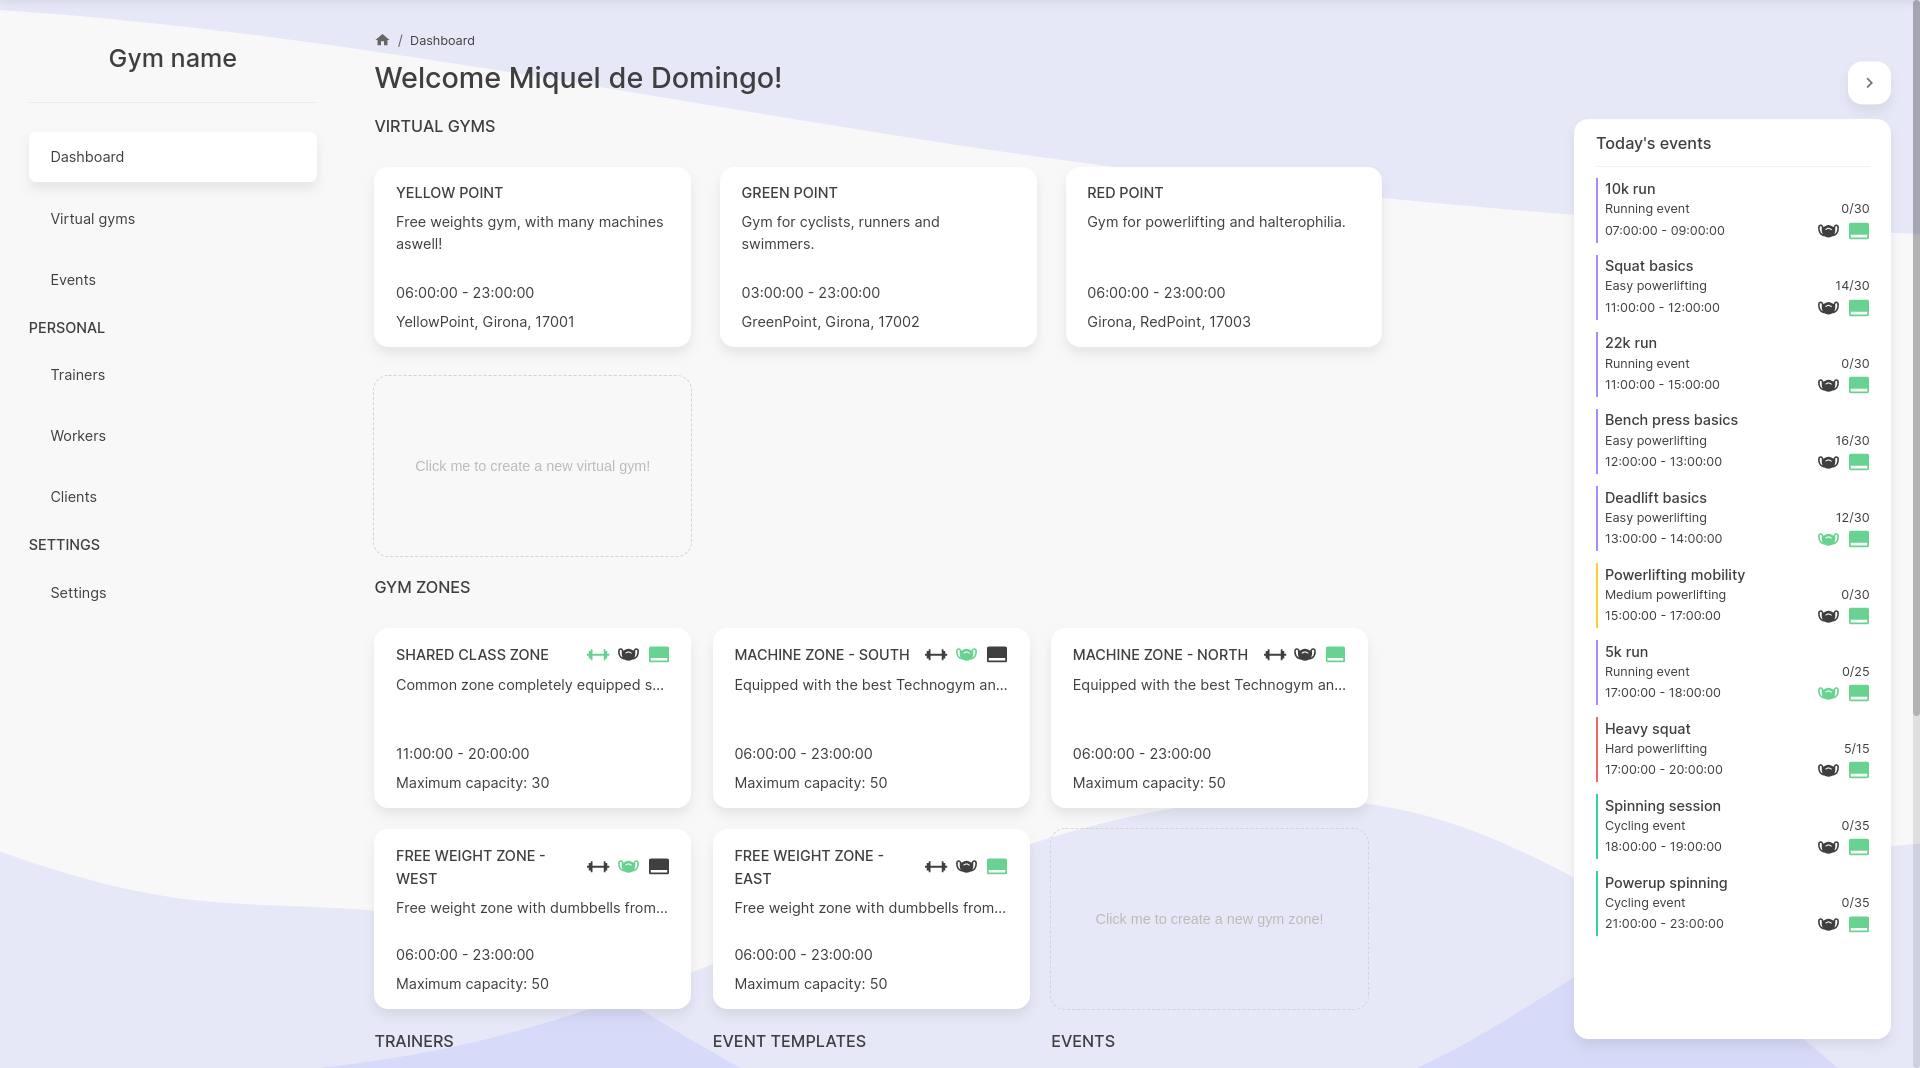
\includegraphics[width=0.65\textwidth]{assets/core-screenshots/dashboard-one.png}
	\caption{Dashboard of the core application from owner's view}
\end{figure}
\begin{figure}[H]
	\centering
	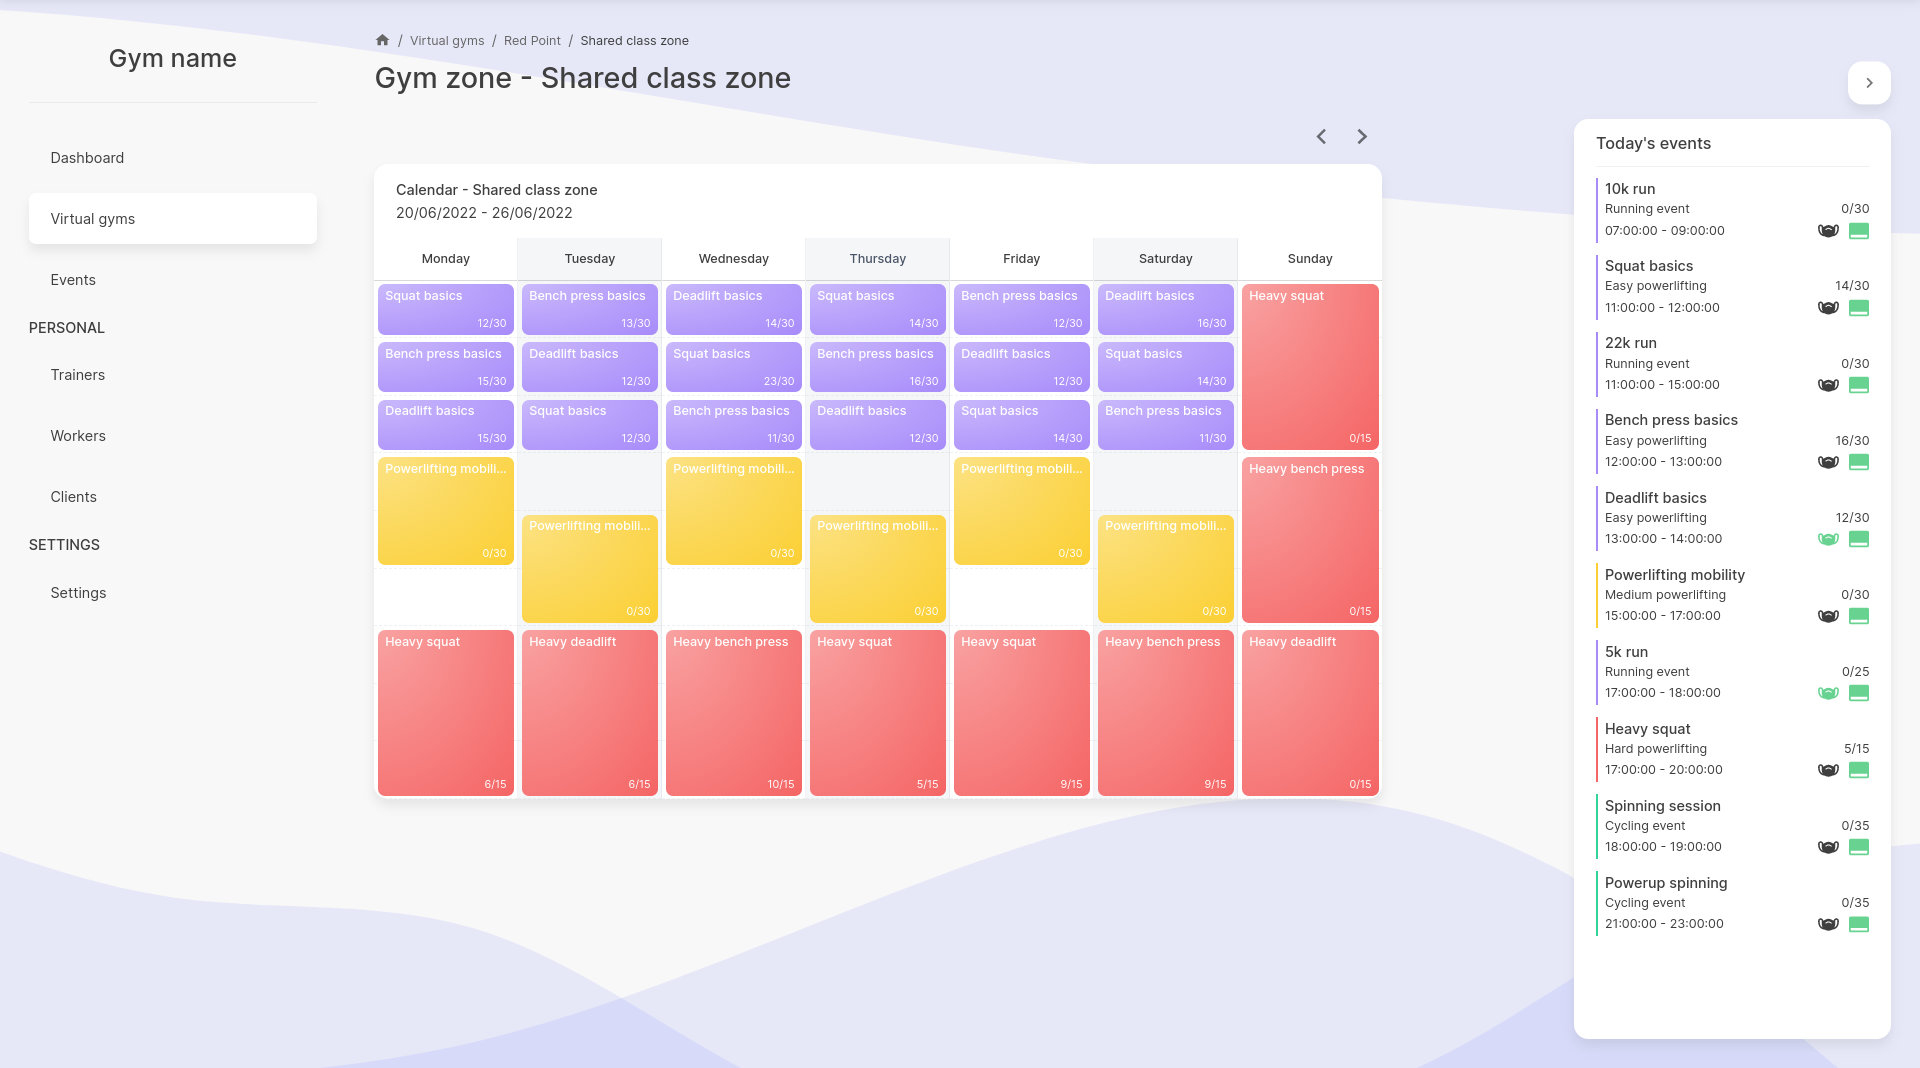
\includegraphics[width=0.65\textwidth]{assets/core-screenshots/gym-zone-two.png}
	\caption{Calendar of a gym zone from owner's view}
\end{figure}
\begin{figure}[H]
	\centering
	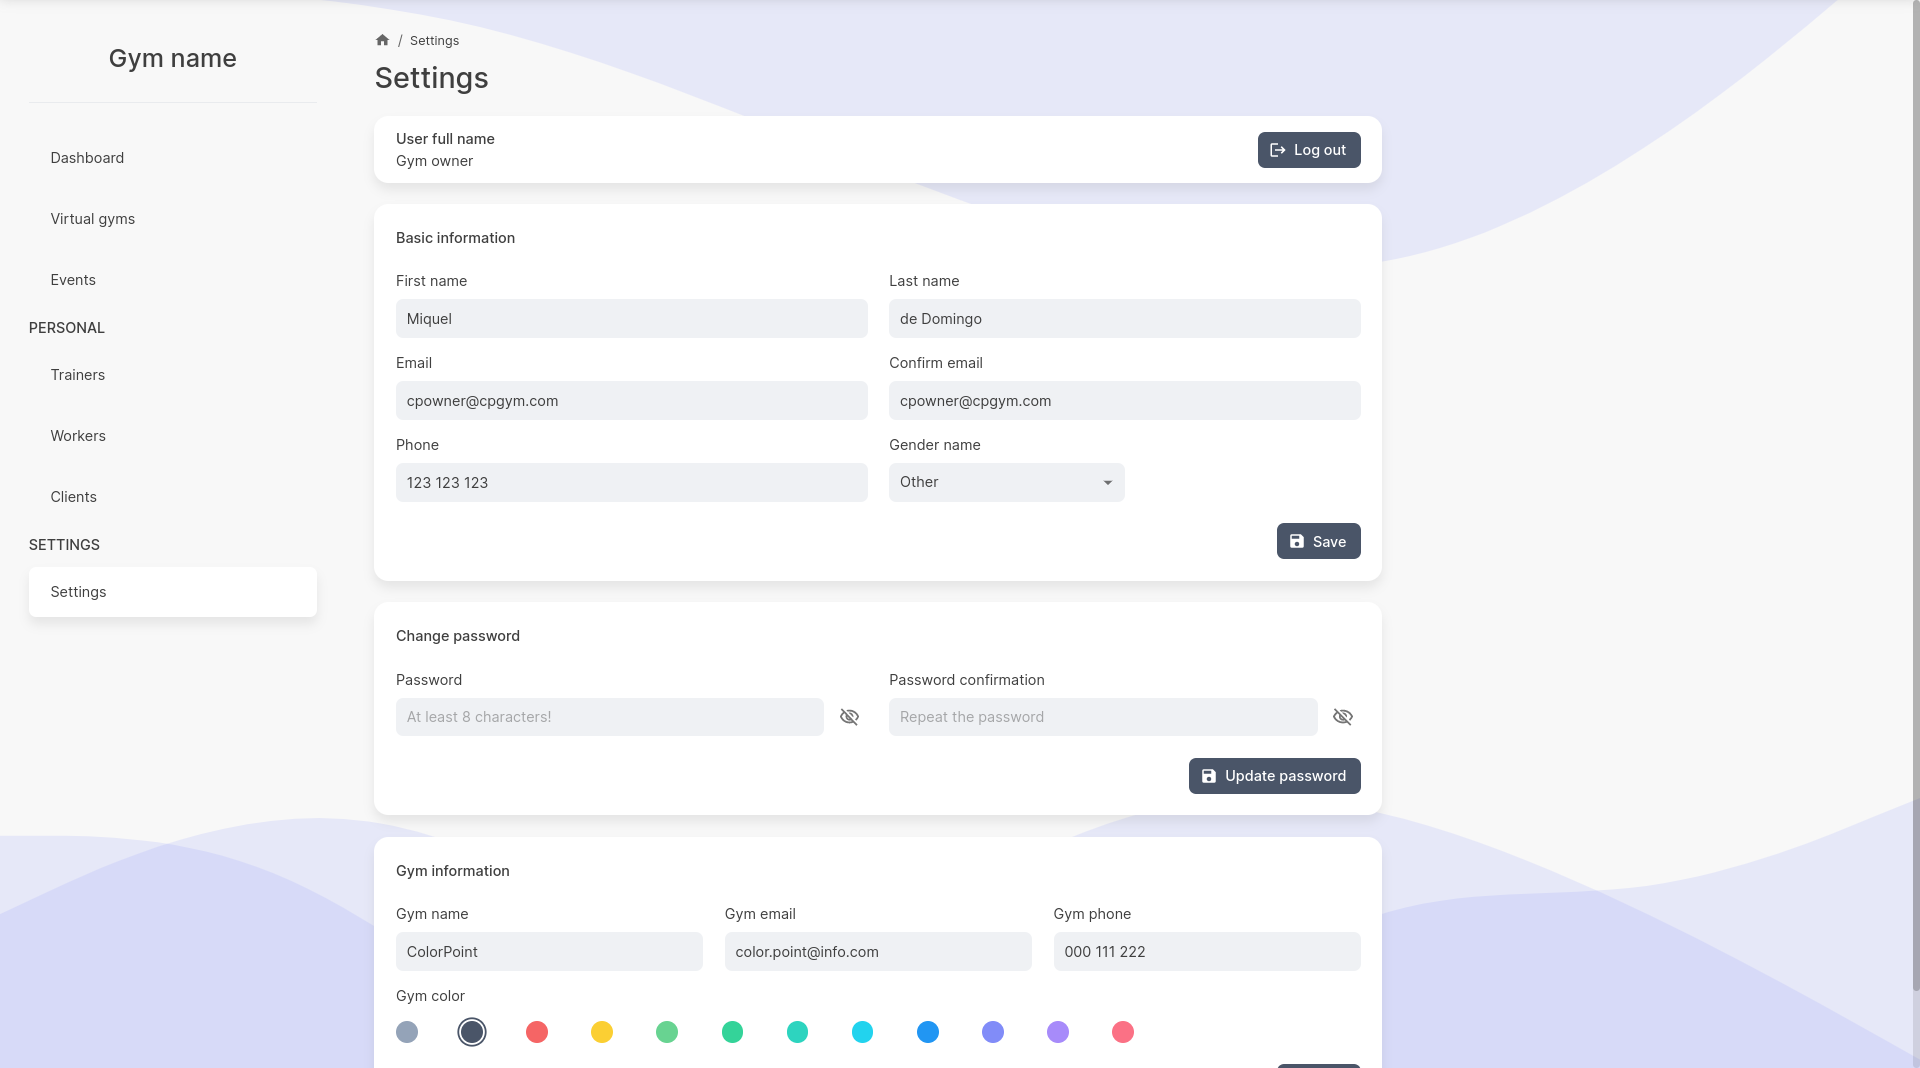
\includegraphics[width=0.65\textwidth]{assets/core-screenshots/settings.png}
	\caption{User settings from owner's view}
\end{figure}
\section{Conclusions}
The goal of the project was to provide a tool that helped both gym owners to manage the appointments their clients made, durign the COVID restrictions. This objective has been accomplished with the Hubbl web application, which allows users to manage appointments in a gym environment. Nevertheless, it is hard to define an app as completely finished, as there may exist a bug that the developers have not seen, or the clients will require new features which will have to be implemented.
\\
It is important to note that one of the objectives of the application was to provide an elegant and sofisticated user experience, at least better than my experience as a user of a similar software. Therefore, the Hubbl application not only provides value with its functionality, but also with the interface and use experience it ships with.
\\
Furthermore, the Hubbl application tries to cover as many aspects as possible, while simplifying the usage of the application. However, there are many other things to improve and to add as new features. Nonetheless, the version that is provided has more than what the app is expected to do. Due to the lack of time, inexpertise in some fields or tools used, and the fact that I have only been developing the application, it has not been possible to develop all that was expected for the wanted deadlines.
\\
The project has required me to use pieces of knowledge acquired in the degree. At the same time, I have been pushed outside my comfort zone, dedicating time to reading documentation pages and similar.
\\
To sum up, the project has provided a sense of how difficult and complex can it be from brainstorming the idea of the application, to finding the proper architecture to later develop it.
\end{document}